\chapter{Introduction}
\label{chap1:introduction}

Since the advent of the Internet, people and companies exchange information on the Web. There is now an abundance of information about a wide range of domains such as science, commerce, leisure, etc. Although the Web browsed by Humans mainly contains unstructured data such as text, a significant amount of structured data exists.

\begin{itemize}
\item hyperlinks from a web page to another in order to point to additional or related information;
\item structural information encoded into the HTML pages using \texttt{table} or \texttt{list} tags for instance;
\item metadata encoded into web pages that provides some meaning about their content.
\end{itemize}

The Semantic Web vision is to enrich this data with machine-readable semantic information, transforming the Web into a global database that we call the \emph{Web of Data}~\cite{bizer:2009:linked}. For example, the description of a table within a web page can be improved by using a semantic markup, e.g., using the RDFa\footnote{RDFa: \url{http://www.w3.org/TR/xhtml-rdfa-primer/}} markup language, so that the columns of the table have a sense: for instance is it concerned with time data, people's name, geographic places, etc.\\

The Semantic Web movement amplified the growth of, now semantically enriched, information on the Web. The Linking Open Data\footnote{\url{http://www.w3.org/wiki/SweoIG/TaskForces/CommunityProjects/LinkingOpenData}} (LOD) project is a successful example, which provides a collection of inter-linked datasets about diverse domains.

A core point of the Semantic Web is the use of ``Uniform Resource Identifiers'' (URIs) for denoting things, e.g., objects, people, places, \ldots. This allows to uniquely name something and describe it, so that it may be reused in other places. Once the data is described using URIs, and also that existing URIs are reused, we reach a state where the data published on the Web is \emph{inter-connected}. The data thus forms a ``graph'', with nodes representing the described objects, and edges detailing the relationship between two objects (nodes).

The inter-connected data is at the ``scale of the Web'', consisting of thousands, if not millions, of different pieces of information about some topics. This scale opens up interesting ways of searching, browsing, and exploring the data.

In order to account for the variety of data about a subject, a ``Data Mashup'' technique is needed as a mean for reading through all different things being said about that subject. Also, within the context of a data mashup, one may be more interested in aggregated measures rather than specific details.\\

Data exploration ultimately requires some knowledge about the \emph{structure} of the (graph) data. There is a need to know what attributes a piece of information contains along with their semantics, so to enable one to search for relevant data. Such knowledge about the structure requires techniques for \emph{managing} the data. In Section~\ref{chap1:introduction:data-mgmt}, we present two data management approaches that are suited to different kinds of data.

The data exploration endeavour is challenged by the scale, heterogeneity, and quality of the data itself. The Web of Data is composed of at least a thousand\footnote{Datahub portal: \url{http://datahub.io/dataset?tags=lod}} of datasets, spanning over a variety of topics. Web Data presents a structure that changes from a dataset to the other, evolving over time. The amount of information about a topic varies from data sources, some being more complete in one aspect and less in another. To overcome these challenges, there is a need for \emph{ranking} the data so that relevant results to an information need are accessed first. This calls for a novel ranking mechanism that leverage the rich structured information of the Web Data; we ponder this in Section~\ref{chap1:introduction:ranking}.\\

Throughout this thesis, we present methodologies designed at shedding light on the structure of Web Data. We propose methods that take into account the shifting nature of the Web Data. We develop then an approach which highlights the ``skeleton'' (structure) of datasets. We leverage the rich structure of the Web of Data in a novel ranking model for (semi-)structured data. We finally present how these techniques can be combined for a more effective exploration of datasets.

In this thesis, we use \emph{Web of Data} to refer to the infrastructure that makes possible the inter-connected (semi-)structured data; and \emph{Web Data} to refer to that (semi-)structured data \cite{delbru:jws:entity}.

%Throughout this thesis, we present methodologies designed at shedding light on the structure of Web of Data. The methods take into account the shifting nature of the Web of Data. We develop then an approach which highlights the ``skeleton'' of datasets. We leverage the rich structure of the Web of Data in a novel ranking model for semi-structured data. We finally present how these techniques can be combined for a more effective exploration of datasets.

\section{Motivation}
\label{chap1:introduction:motivation}

%- difficulty of formulating queries and data integration from multiple sources
%	- unknown data structure: what vocabulary(ies), what predicate is used, which predicate is relevant
%	- data heterogeneity: data comes from a variety of sources with different schema. the ontology does not help here to know the structure!
%	- structure inconsistency: not all entities have the same set of properties, even if they are of the same type.
%		- makes the query more complex since we need to account for missing properties
%		- should a structure description reflect this fact ? This has impact on the space needed for that description.
%
%- ranking of graphs
%	- ranking model retains or not the structure
%	- due to the data heterogeneity, an attribute of a concept may have several values. How to cope with this ?
%	- because of the graph structure of the ranked documents, the rank of a document depends on the rank of some related entities. Bring a parallel with PageRank ? Maybe not, this is the opposite: the parent score is dependent of the child's score.
%	- challenge of data structure inconsistency
%	- ranking model needs to be data structure agnostic
%	- position of keywords occurrences in the graph is important

A user with an information need has at his disposition several ways to find relevant data. A search engine may be used so that documents embedding relevant, structured data, can be retrieved: for example, thanks to services such as Swoogle~\cite{ding:2004:ssm} or Sindice~\cite{oren:2008:sdl}. Such engines provide search access using Information Retrieval indices, on which boolean queries are evaluated.

However, it is better to rely on graph query languages such as the standardised SPARQL\footnote{SPARQL: \url{http://www.w3.org/TR/sparql11-overview/}} language, if the user's quest requires more expressivity than what is possible with boolean queries. In such a case, a direct access to the data is needed. Platforms such as DataHub\footnote{DataHub: \url{http://datahub.io/}} or Publicdata\footnote{PublicData.eu: \url{https://publicdata.eu/}} present available data accesses, e.g., download of data dumps or a SPARQL endpoint. Once a user has found a possibly relevant dataset, he has the actual daunting task of querying that dataset: not because of the language itself, but due to the lack of information about the dataset's structure.

As an illustration, we consider the Eunis\footnote{Eunis on DataHub: \url{http://datahub.io/dataset/eunis}} dataset which contains information about species and their habitats.

\paragraph{Query formulation.}

Although the Eunis dataset can be considered as a small dataset, a user is nonetheless challenged in effectively and efficiently querying the dataset. In order to formulate a query, predicates and/or types occurring in the dataset are needed. However, such information is in general not available. Here, a VoID~\cite{alexander:2009:dld} description is present, but that specific file does not provide sufficient information beyond what is needed for simple queries.

A simple way to retrieve such information is to query the dataset directly. However, we then have to choose among 500 types and at least 1500 predicates. The Eunis dataset exhibits as well the use of over 40 different vocabularies. A possible reason of such heterogeneity can be that the Eunis dataset is the end result of several integrated data sources. Also, as a consequence of this heterogeneity, a single ontology cannot help in learning about the dataset's structure.

As the query construction progresses, the user needs to know which predicates/types can be used in \emph{conjunction} with the already selected ones. At this point, a user is faced with the issue of data \emph{inconsistency}: the resources in a datasets do not all share the same set of predicates/types. Thus, the query must be carefully built so to retrieve actual results. The complexity of writing the query increases since the user needs to account for missing predicates (or types). \textit{How can the user learn about the data structure so to formulate intelligent queries ?}

\paragraph{Ranking.}

With the Eunis dataset having at least 500 types and 1500 predicates, the user is left with the challenge of deciding which one to use. Are the ones most used the more relevant for the user ? Does the predicate label, e.g., \url{http://xmlns.com/foaf/0.1/name}, give some indication about the semantic of that predicate ? One may dereference it and read its description, but this demands yet additional work for the user. \textit{How can a user decide which type/predicate to use ?}

\section{Data Management}
\label{chap1:introduction:data-mgmt}

Web Data is composed of a variety of data about many entities, for example which can be a person\footnote{\url{https://en.wikipedia.org/wiki/Buzz_Aldrin}}, a country\footnote{\url{https://en.wikipedia.org/wiki/Ireland}}, an event\footnote{\url{https://en.wikipedia.org/wiki/Moon_landing}}, etc.
The decentralised nature of the Web has the effect that information about a same \emph{entity} is available on several web pages. Data sources can be complementary in some aspects, and redundant in others. Furthermore, each source has its own take on data modelling. Sources may label an attribute of an entity differently although what is described is the same. Sources may also represent an attribute differently, e.g., the name of a person as two properties with first and last name, versus a single property which is a concatenation of the two. These facts highlight the \emph{heterogeneity} of the data on the Web, which stands as a challenge when managing data.\\

In order to fulfill an information need, a user generally uses a web search engine. This allows him to browse only the most relevant pages with regards to his need out of the billions of web pages that the Web consists of. To achieve this, search engines rely on the structure of the data so to rank documents appropriately. The knowledge of the structure of the data, which can sometimes be seen as a \emph{schema}, is a necessary medium for exploration and, ultimately, finding the answer to one's need.

To ease this process, many vocabularies have been built over the years for representing one's data; for example the following:
\begin{labeling}{\textbf{FOAF}}
	\item[\textbf{FOAF}\protect\footnotemark] defines terms for describing a person and the relationships between people;
	\footnotetext{\url{http://xmlns.com/foaf/spec/}}
	\item[\textbf{SKOS}\protect\footnotemark] is used for representing knowledge organisation systems such as taxonomies; or
	\footnotetext{\url{http://www.w3.org/2009/08/skos-reference/skos.html}}
	\item[\textbf{GEO}\protect\footnotemark] represents geospatial coordinates.
	\footnotetext{\url{http://www.w3.org/2003/01/geo/wgs84\_pos}}
\end{labeling}

However, vocabularies tend to be loosely followed in datasets --- this is reflected by the disparate use of vocabulary terms and ontologies across datasets in \cite{campinas:2011:eos}. One of the reasons is that many different design choices are possible while modelling one's data. The structure of the data and use of vocabularies evolve over time as new requirements come: new terms are added, some are deleted, and the semantic of some may be modified. Furthermore, changes in the vocabulary upstream may not be reflected in the datasets in which it is used. As a consequence, we refer to Web Data as being \emph{semi-structured}~\cite{abiteboul:1997:icdt}.\\

The vocabulary heterogeneity, combined with the scale of datasets, actually complicates the effective use of the data. This calls for novel techniques designed at ``understanding'' the data while taking into account its structural richness.

\subsection{Schema-based Data Management}

In the relational database community, a \emph{logical schema} provides an overview of a database. The schema describes the content of the database, how it is structured and what attributes it has. In the Web of Data, such a description is generally not available, thus preventing an effective exploration of the data.

Web Data is in general not bundled with a schema, or a description akin to a schema. This is due to the very nature of Web Data: it is dynamic, diverse, and ever-evolving. The growth of Web Data is in essence similar to that of the Web: it evolves organically, constrained by nothing specifically. In such an environment, a schema-based data management is extremely difficult to put into place, if not impossible.

\subsection{Decentralised Data Management}

Web Data can be created without the need to follow specific rules. The data does not need to adhere to some kind of pre-defined schema. Inter-linking with others' data is promoted in the Web of Data by the use of URIs. The distributed aspect of the data is emphasised by Halevy et al.~\cite{halevy:2003:smp} where a peer-to-peer data management system is proposed. However, data sources are assumed to have a schema, and the existence of a global schema that \emph{mediates} the sharing of information between sources is needed.

In the Web of Data, the existence of a central place where the schema of data sources is kept is unreasonable due to the scale and dynamicity of the data.
Nonetheless, a schema enables two benefits
\begin{inparaenum}[(1)]
\item it ensures that new data adheres to that schema; and
\item it provides an overview over existing data.
\end{inparaenum}
Given that the first point cannot be achieved in the Web of Data context, we propose the graph summary as a way to provide the second point: it is a novel system for managing distributed, heterogeneous data sources on the Web.

%\section{Graph Exploration}
%
% In order to put this information into use, there exists several approaches that range from manual to supervised exploration.
%
%\subsection{Follow-Your-Nose}
%
%Graph data can be explored by going from node to node, where a node provides more information about a concept related to the originating node. In the Web of Data, this is done by looking up URIs\footnote{\url{http://www.w3.org/wiki/FollowLinksForMoreInformation}}. However, this approach presents scalability and trust issues. The number of resources in the Web of Data is overwhelming and so the number of data to look up grows exponentially. Also, the data retrieved by following a link can be questionable regarding its accuracy. This approach starts with a set of seed URIs, which poses the challenge of choosing which URI to choose. The follow-your-nose paradigm can be used at query-time~\cite{hartig:2009:esq} for finding potentially relevant data.
%
%\subsection{Keyword-based Exploration}
%
%Web search engines are used for browsing a large set of documents which are retrieved based on a keyword query. The documents are then ranked based on how relevant they are with regards to the query. A similar line of thought is followed for browsing the Web of Data~\cite{ding:2004:ssm,cheng:2008:fsb,oren:2008:sdl}. These services provide an index of documents embedding structured data, e.g., RDFa. Documents are retrieved by querying for a specific URI or by passing a complex boolean query. Such systems are useful in locating documents that can be used as seeds for deeper exploration. Although keyword queries allow for a quick loop up of documents, they do not consider the rich structure of documents. Complex queries can be expressed using systems like Sindice~\cite{oren:2008:sdl}, but this assumes that the schema of relevant documents is partially known.
%
%\subsection{Metadata-based Exploration}
%
%The exploration of data can be performed at different levels of abstraction. At the lowest level, the browsing focuses on the resources. At the highest level, the browsing is done over datasets, where a dataset represents a sub-graph of the Web of Data. At that level, information about a single resource is of little to no importance. The information need in this case is a concept that refers to a group of resources. Metadata information about datasets is then needed to understand their content or what kind of information they have available. Different approaches have been proposed for describing the content and structure of datasets~\cite{alexander:2009:dld,konrath:2012:schemex}. which can then be used to facilitate the discovery of datasets \cite{akar:2012:ldow,konrath:2012:schemex}.

\section{Ranking of Web Data}
\label{chap1:introduction:ranking}

With the growth of the Web in the early days of The Internet, the use of web search engines to sift through the mass of documents marked a significant milestone in the interaction of people with regards to data. Then, the ability of search engines not only to retrieve but also to \emph{rank} the data by relevance to a query marked another milestone: the possibility to find a needle in the haystack.

Traditionally, the documents ranked contain mostly textual information, with little structure that can be leveraged by a ranking algorithm. Web documents contain HTML markup for display purposes, but those can be cues for the importance of a piece of text within the document. Web Data instead is structured beyond what can be extrapolated from the markup cues. Therefore, this calls for a novel ranking mechanism that supports this rich structure.

\subsection{Traditional Ranking on The Web}

Documents on the Web are mainly textual, containing information only for Humans to process. In order to rank such documents, a straight-forward approach is to consider a document as a set of words and using word frequencies to estimate its importance within the document. Thus, with such a modelling a document is referred to as a \emph{bag of words}.

The ranking of a document can be improved by, for example, adding some structural information into the algorithm. Some specific parts can be extracted so to apply a weight, for instance the title. Such approaches are referred to as \emph{\gls{field}-based} ranking. However, the structure considered in those are too simple and so they cannot leverage the complex (graph) structure that is exhibited in Web Data. This marks a shift from the ranking of (\gls{field}-based) documents to graph data.

\subsection{Ranking of Graph Data}

In the Web of Data, we use URIs to name things, e.g., people, monuments, places, \ldots, which allows one to lookup an URI and learn about it, but also for others to reference that URI in their own dataset. The Web Data takes then the form of a graph, where a node represent a concept and the edge a labelled relationship that links two nodes.
While Web Data follows the standard RDF format that opens many opportunities to tackle graph ranking, we consider in this thesis to improve the ranking model.

In Web Data, the structure of the graph carries some information about the data. However, most of it is discarded by \gls{field}-based ranking approaches due to the bag of words modelling. The Figure~\ref{chap1:introduction:fig:bow-graph} depicts a  graph about ``Ireland'' and its neighbouring country; the Figure~\ref{chap1:introduction:fig:bow} is a depiction of its bag of words. We observe that with the bag of words modelling, we lose some semantic that is carried by the structure: the population number is not closely associated with the ``United Kingdom'' anymore.

The ranking of a graph requires a novel way of modelling the data that does not discard the structure.
Hence, we propose the \emph{``MF'' ranking model} that leverage the graph structure in order to better compute the relevance of a graph with regards to a query.

\begin{figure}
	\centering
	\begin{subfigure}[b]{0.45\textwidth}
		\centering
		\resizebox{\textwidth}{!}{
			\begin{tikzpicture}[->,>=stealth',node distance=3cm]
\node[draw,circle] (a) {ex:1};
\node[draw,right of = a] (b) {Country};
\node[draw,above right of = a] (c) {Ireland};

\node[draw,circle,below right of = a] (d) {ex:2};
\node[draw,right of = d,xshift=1cm] (e) {United Kingdom};
\node[draw,below right of = d] (f) {64.1 M};

\path[every node/.style={fill=white,font=\footnotesize}]
(a) edge node {is\_a} (b)
(a) edge node {label} (c)
(a) edge node {neighbour} (d)
(d) edge node {label} (e)
(d) edge node {population} (f)
;
\end{tikzpicture}
		}
		\caption{A simple graph}
		\label{chap1:introduction:fig:bow-graph}
	\end{subfigure}
	\qquad
	\begin{subfigure}[b]{0.45\textwidth}
		\centering
		\resizebox{\textwidth}{!}{
			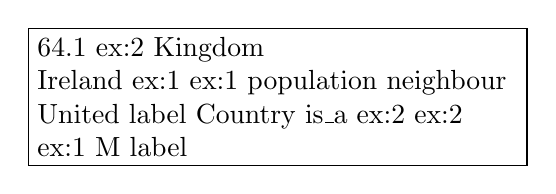
\begin{tikzpicture}
\node[draw,text width=6.1cm] {
64.1 ex:2 Kingdom \newline
Ireland ex:1 ex:1
population neighbour United
label Country is\_a
ex:2 ex:2 ex:1 M label
};
\end{tikzpicture}
		}
		\caption{Bag of words modelling}
		\label{chap1:introduction:fig:bow}
	\end{subfigure}
	\caption{A graph modelled as a bag of words}
\end{figure}

\section{Challenges}

The purpose of the summary is to describe the structure of a graph. Therefore, it can hold the function of a \emph{schema} for that graph.
A schema is the basis of many algorithms over the data. A schema describes the content thus facilitating users to search for a particular resource. From the description a schema provides, one may draw out statistical information about the data that can be useful in some scenarios, e.g., query optimisation. Schemas help in the integration process of several data sources. As a consequence, a major challenge is to determine what features of the data can be used in order to effectively generate a schema. We study this aspect in Chapter~\ref{chap4:summary}.\\

The construction of a graph summary does not ensure that the entity graph can be re-built from its summary. This means that some details about the structure of the graph was discarded during the summarisation process. Although some errors in the summary can be acceptable for a user exploring the data, it can cause a significant drop of performance for a query optimizer. Hence, it is necessary to measure how accurate a summary is with regards to the data. We introduce a model for measuring the precision of a summary in Chapter~\ref{chap5:precision}.

In the recent years, the amount of data has been growing increasingly. A glimpse of this growth over the years can be visually appreciated\footnote{The Linking Open Data cloud diagram: \url{http://lod-cloud.net/}} through the many diagrams of the Linking Open Data cloud. It is common to see data with millions of entities and billions of statements, to which the ``Open Data'' movement contributed a significant part. However, the ease of sharing data has the downside of that data not following a strict schema, if any.\\

As a consequence, there is a need for techniques that can provide a structure akin to a schema, e.g., a summary, without restraining the ``evolution'' of the data, while at the same time that can scale to large volumes of data.

\section{Scope of the Research}

The scope of this thesis is to study the creation of summaries on large scale semi-structured information sources. By semi-structured, we mean data that presents some structure but that is not followed strictly by all records in the dataset. By large, scale we mean data which contains millions of entities with billions of statements describing said entities.

The main challenge is to present a summary creation process that is able to cope with the scale of the data, as well as with the variability of the data due to the heterogeneous and loose use of vocabularies. To this end, we investigate graph summarisation approaches which generate summaries via graph homomorphism. Due to the heterogeneity of the data, the generation of \emph{approximate} summaries is the only viable option for a large number of use cases.

Different applications have varying interactivity with respect to the summary. We investigate ranking techniques for retrieving first the parts of the summary an application need. We evaluate how ranking can be used for improving the exploration of data.

\section{Applications}

Graph summarisation produces a \emph{summary} of the structure of the graph, providing information akin to a schema in relational databases. We can then leverage the summary in several ways, of which some are presented in this thesis.

\begin{labeling}{\emph{Browsing of a dataset's structure.}}
\item[\emph{Graph schema.}] We present in Section~\ref{chap7:applications:wdm} that the graph summary can serve the function of a \emph{schema} for the graph. The generated summary of a graph highlights its structure, unveiling the underlying schema; ultimately this allows one to query for the desired information.
\item[\emph{Querying assistance.}] In Section~\ref{chap7:applications:sparqled:recommendation} we use the structural information from a summary in order to assist a user in writing a query over the graph. This allows users having little to no knowledge about the data to build meaningful queries.
\item[\emph{Browsing of a dataset's structure.}] The information gathered during the graph summarisation process of a dataset is made available for browsing in Section~\ref{sec:web-data-inspector}. This enables a user to learn about the internals of a dataset: its structure, the kind of information it carries, the relationships between concepts, or its connections to other datasets. With such knowledge, the user may identify problems with the data, e.g., missing attributes.
\end{labeling}

\section{Scientific Methodology}

We deployed several scientic methods from different fields from Computer Science, especially \emph{theoretical} Computer Science and \emph{experimental} Computer Science.

Specifically, we investigated several graph summaries useful for different aspects. We then generalised these to define a general formal framework, described in Chapter~\ref{chap4:summary}, to cover approximate graph summaries as well. We determined the complexity of the resulting algorithms and evaluated their behaviour in experimental settings in Chapter~\ref{chap5:precision}.

We also experimented with the resulting graphs to investigate the behaviour in a practical setting within the Sindice~\cite{delbru:jws:entity} project and evaluated the results.

The Sindice~\cite{delbru:jws:entity} project aimed to create an Information Retrieval search engine for Web Data. That engine had already collected a significant amount of data, but then with this came the challenge of writing meaningful queries. To help with this need, a good ranking is needed which was investigated in~\cite{delbru:2010:hierarchical} and continued with the MF ranking model (Chapter~\ref{chap6:ranking}). Difficulty to understand what was inside the collected data, but also the challenge with writing queries motivated the research into graph summarisation (Chapter~\ref{chap4:summary}).

\section{Outline}

The thesis is divided in three parts. This first part \emph{Background} contains the introduction to the thesis, and presents fundamental concepts and models that will be reused throughout the rest of the thesis. We introduce in the second part \emph{Methods} new techniques for generating and evaluating graph summaries, as well as a new ranking model for semi-structured data. In the final part \emph{Putting the Pieces Together}, we describe applications of the presented methods.

\minisec{Part II: Foundations}

\begin{labeling}{Chapter~\ref{chap2:semi-structured-data}:}
\item[Chapter~\ref{chap2:semi-structured-data}:] We present here a graph data model that encompasses the wide variety of formats used for modelling structured data. The model is layered so to represent the concepts of entity and dataset.% Then we describe a graph schema model which fits between those two layers.
\end{labeling}

\minisec{Part III: Methods}

\begin{labeling}{Chapter~\ref{chap4:summary}:}
\item[Chapter~\ref{chap3:review}:] We present in this chapter several approaches at summarising graph data and for what scenario they were built for. We emphasize their shortcomings and how these are answered thanks to the graph summary.
\item[Chapter~\ref{chap4:summary}:] In this chapter, we introduce the formal model of a graph summary. Then, we present a technique for generating graph summaries for Web Data at scale.
\item[Chapter~\ref{chap5:precision}:] The summary of a graph is built in a bottom-up fashion, through the aggregation of nodes of the entity graph. The graph summary being a graph homomorphism, it is not assured that entity graph can be re-built from its summary. Therefore, some details about the structure of the graph are missing from the graph summary. In order to account for this loss, we developed a model for measuring the precision of a graph summary.
\item[Chapter~\ref{chap6:ranking}:] In this chapter, we introduce the ``MF'' ranking model for semi-structured data. The model considers the structural heterogeneity of the data for a better scoring of entities.
\end{labeling}

\minisec{Part IV: Putting the Pieces Together}

\begin{labeling}{Chapter~\ref{chap7:applications}:}
\item[Chapter~\ref{chap7:applications}:] In this chapter, we present applications of the introduced methods. We develop a system based on a generated graph summary that assists users in writing graph-shaped queries without a priori knowledge of the data structure. We present an RDF model of the graph summary, which allows the summary to serve the function of a schema. In addition, we present another application of the graph summary that enables one to inspect a dataset so that problems with the data may be identified.
\end{labeling}

\section{Contributions}

Web Data is a large collection of (semi-)structured data about a variety of domains. The data comes from a wide panel of sources, ranging from database dumps to publicly-edited content. In order to use this information effectively, it is necessary to know how the data is structured, which is essential in cases such as data integration or querying for example. In the context of Web Data, the availability of such a description of the data structure is extremely rare.

The main contribution of this work is we believe a solution to this basic challenge when interacting with Web Data: a method for extracting the structure of large and distributed semi-structured datasets through graph summarisation. Since this method needs to scale to large datasets, we investigate extracting an approximation of the data structure. As a consequence, we also investigate the use of a ranking data model in order to reduce the loss of precision due to the approximation.

Specific contributions include:
\begin{itemize}
	\item a formal model for an entity graph in Chapter~\ref{chap2:semi-structured-data};
	\item a review of literature regarding the summarisation of graphs in Chapter~\ref{chap3:review};
	\item a method for generating graph summaries of large and distributed semi-structured data in Chapter~\ref{chap4:summary}, based on the work in \cite{campinas:2012:dexa,campinas:2013:efficiency};
	\item a model for measuring the precision of a graph summary in Chapter~\ref{chap5:precision}, based on the work in \cite{campinas:2013:efficiency};
	\item a novel ranking model specifically designed for dealing with the structural and content heterogeneity of Web Data in Chapter~\ref{chap6:ranking}, based on the work in \cite{campinas:2011:semsearch,campinas:2012:bm25mf}; and
	\item a set of tools for improving the exploitation of semi-structured data in Chapter~\ref{chap7:applications}, based on the work in \cite{auer:2014:linked}.
\end{itemize}
